\part{Causal analysis and Logic programming - Daniele Meli}
\section{Introduction \& Motivation}
AI (and particularly ML) can solve very complex problems in real life such as: Autonomous vehicles, Industrial automation and robotics Medical imaging and diagnosis ecc..
The problem with most of the ML models is that they are black boxs i.e we cannot understand the motivation behind the output.\\

The goal of Explainable AI (XAI) is to explain the behaviour of AI systems, in order to increase the
level of understanding and \emph{trust}. 
\begin{figure}[H]
    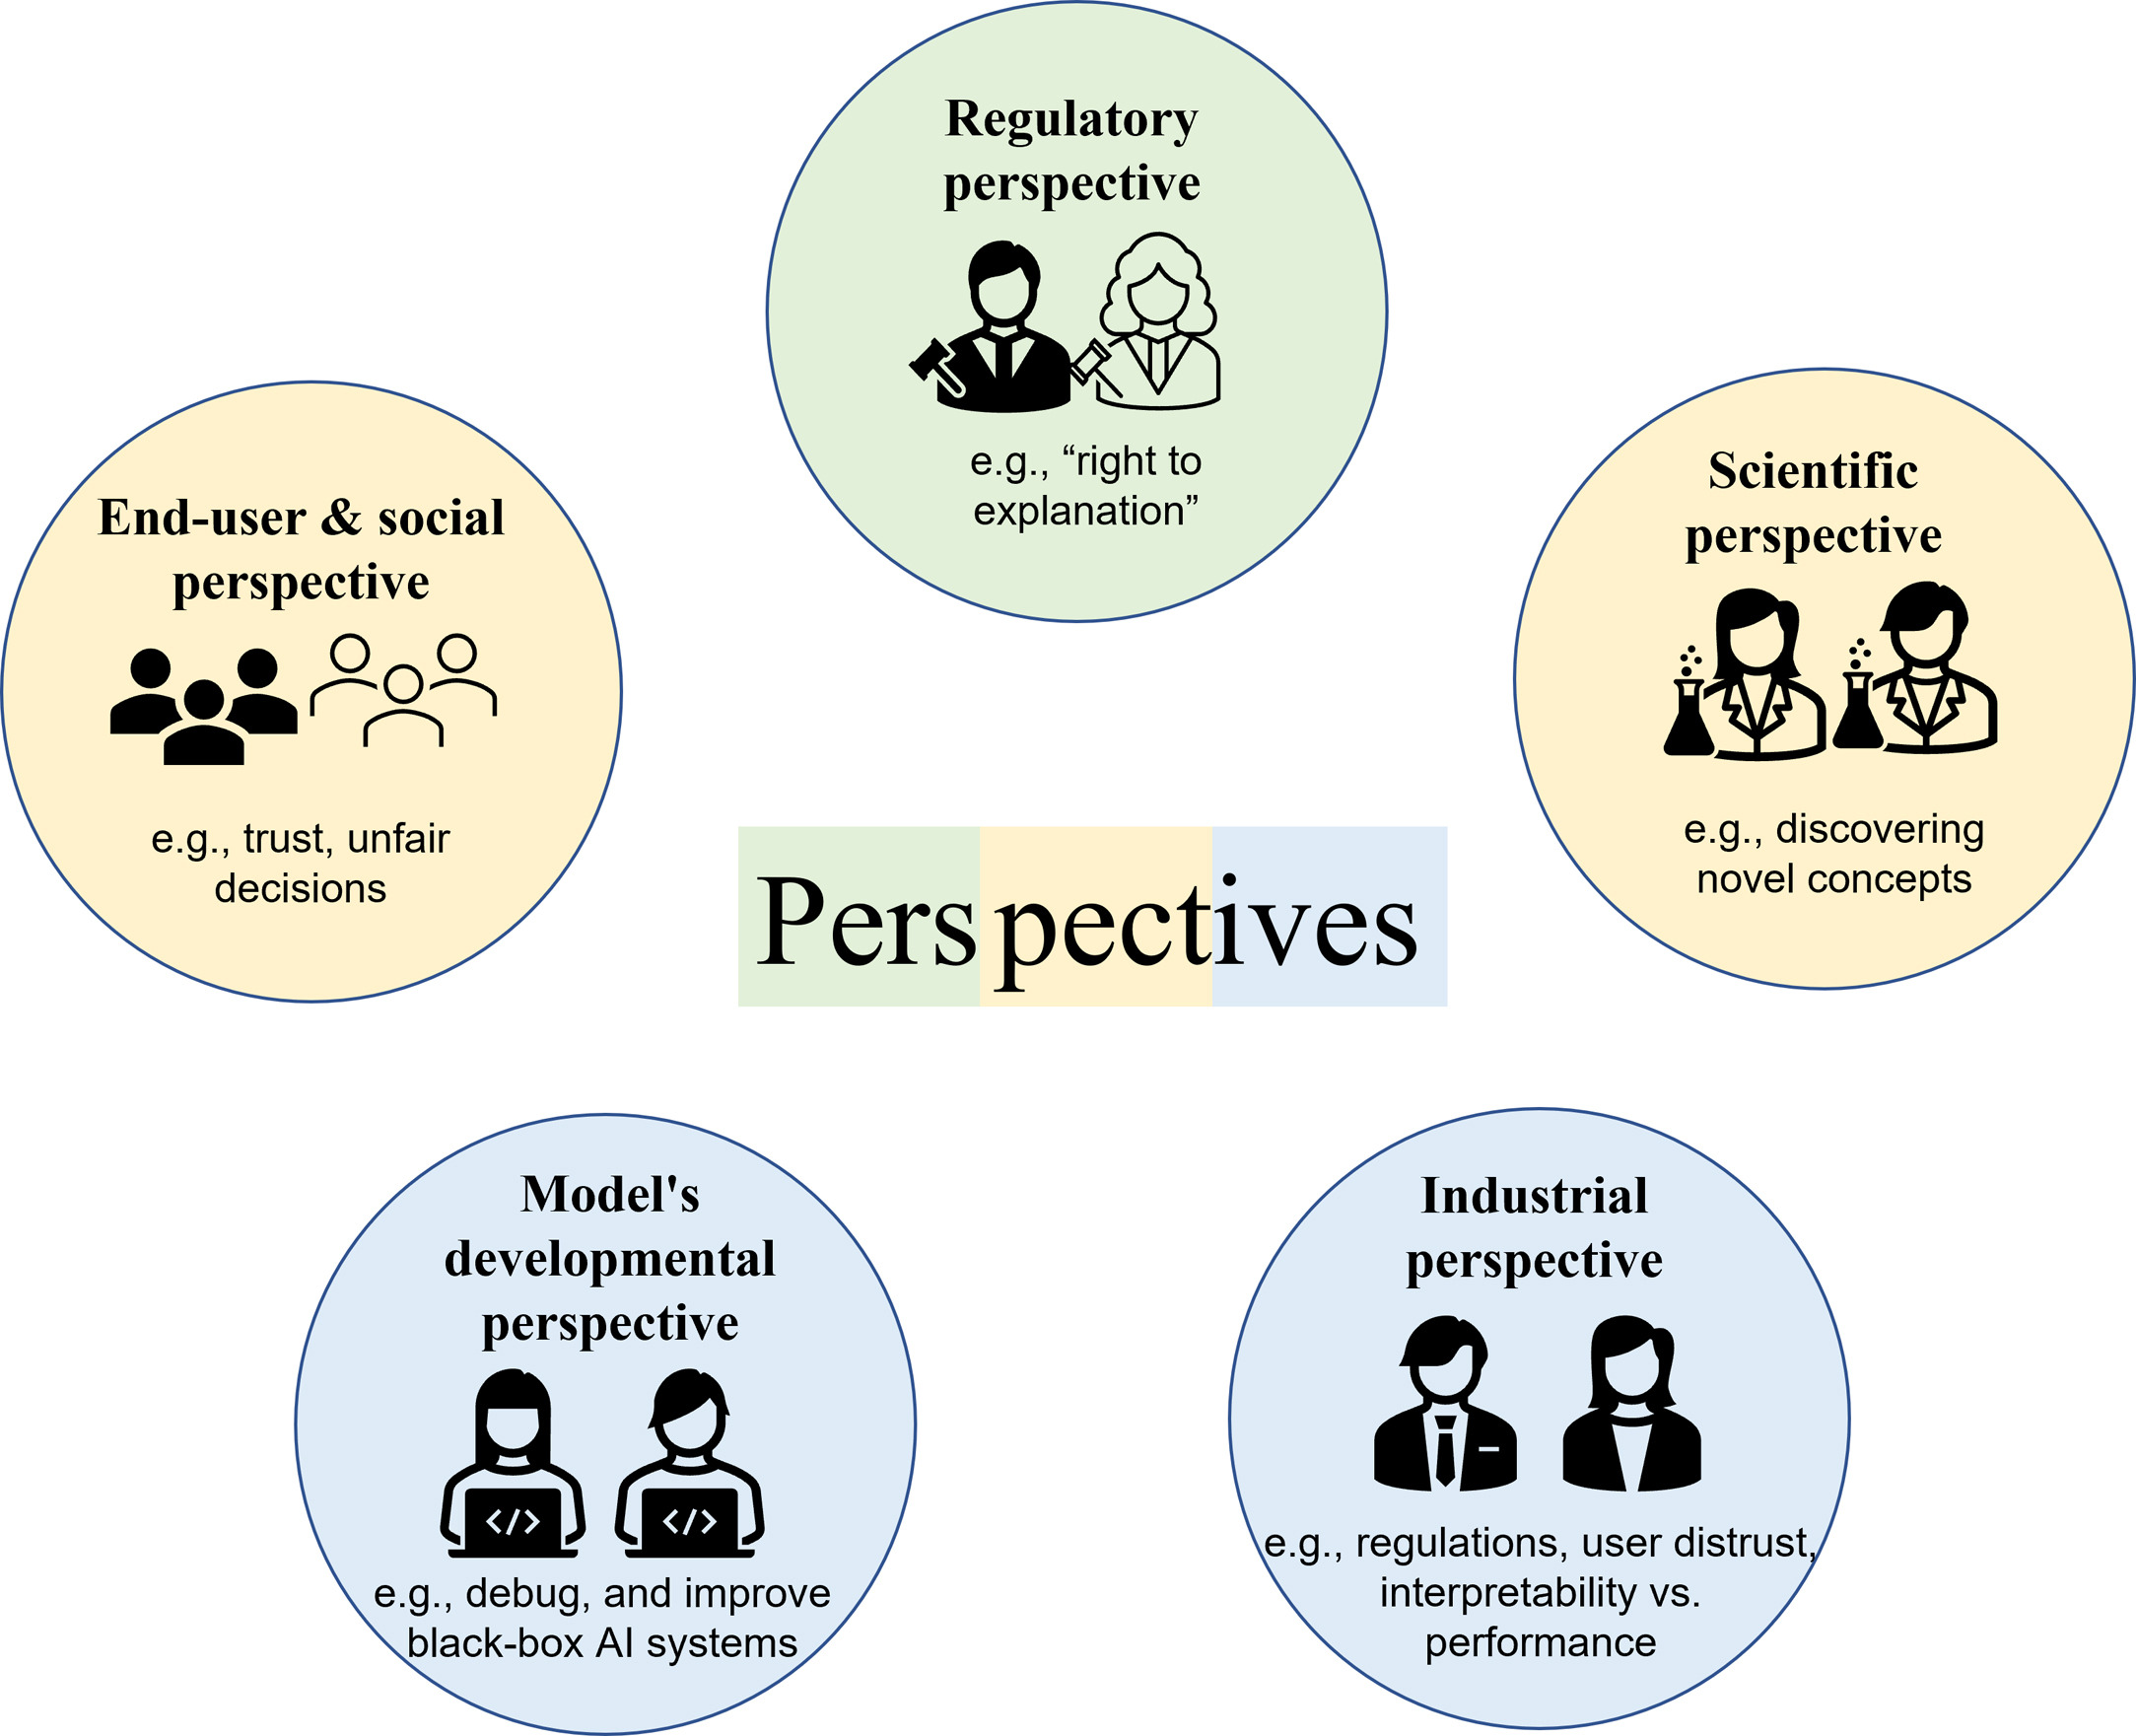
\includegraphics[width=0.5\textwidth]{img/motivation.jpg}
    \centering
    \caption{Summary of the main motivations regarding the use of XAI}
\end{figure}
We can summarize the motivation into 5 main points:
\begin{enumerate}
    \item Regulatory Perspective
    \item Scientific Perspective
    \item Industrial Perspective
    \item Model's developmental perspective
    \item End-user and social perspective
\end{enumerate}
\subsection{Motivation}
\subsubsection*{Regulatory Perspective}
Black-box AI systems are being utilized in many areas of our daily lives, which could be resulting in unacceptable decisions, especially those that may lead to legal effects. 
The European Union's General Data Protection Regulation (GDPR)\footnote{\url{https://www.privacy-regulation.eu/en/r71.htm}} is an example of why XAI is needed from a regulatory perspective. 
These regulations create what is called the \emph{right to explanation}, by which a user is entitled to request an explanation about the decision made by the algorithm that considerably influences them.

\subsubsection*{Scientific Perspective}
When building black-box AI models, we aim to develop an approximate function to address the given problem. 
Therefore, after creating the black-box AI model, the created model represents the basis of knowledge, rather than the data. 
Based on that, XAI can be helpful to reveal the scientific knowledge extracted by the black-box AI models, which could lead to discovering novel
concepts in various branches of science.

\subsubsection*{Industrial perspective}
Regulations and user distrust in black-box AI systems represent challenges to the industry in applying complex and accurate 
black-box AI systems. Less accurate models that are more interpretable may be preferred in the industry because of regulation
reasons. A major advantage of XAI is that it can help in mitigating the common trade-off between model interpretability and performance,
thus meeting these common challenges. 
However, it can increase development and deployment costs.

\subsubsection*{Model's developmental perspective}
Several reasons could contribute to inappropriate results for black-box AI systems, such as limited training data, biased training data, outliers, adversarial data, and model overfitting. 
Therefore, what black-box AI systems have learned and why they make decisions need to be understood, primarily when they affect humans lives. 
For that, the aim will be to use XAI to understand, debug, and improve the black-box AI system to enhance its robustness, increase safety and user trust, and minimize or prevent faulty behavior, bias, unfairness, and discrimination.

\subsubsection*{End-user and social perspective}
In the literature of deep learning, it has been shown that altering an image such that humans cannot observe the change can lead the model in producing a wrong class label (Adversarial Attacks). 
On the contrary, completely unrecognizable images to humans can be recognizable with high confidence using DL models.
Such findings could raise doubts about trusting such black-box AI models. 
The possibility to produce unfair decisions is another concern about black-box AI systems. 
This could happen in case black-box AI systems are developed using data that may exhibit human biases and prejudices.
Therefore, producing explanations and enhancing the interpretability of the black-box AI systems will help in increasing trust because it will be possible to understand the rationale behind the model's decisions, and we can know if
the system serves what it is designed for instead of what it was trained for. Furthermore, the demand for the fairness of black-box AI systems decisions, which cannot be ensured by error measures, often leads to the need for
interpretable models.

% \part{title}
\subsection{XAI - One topic, two keywords}
\begin{minipage}[c]{0.3\textwidth}
    \begin{figure}[H]
        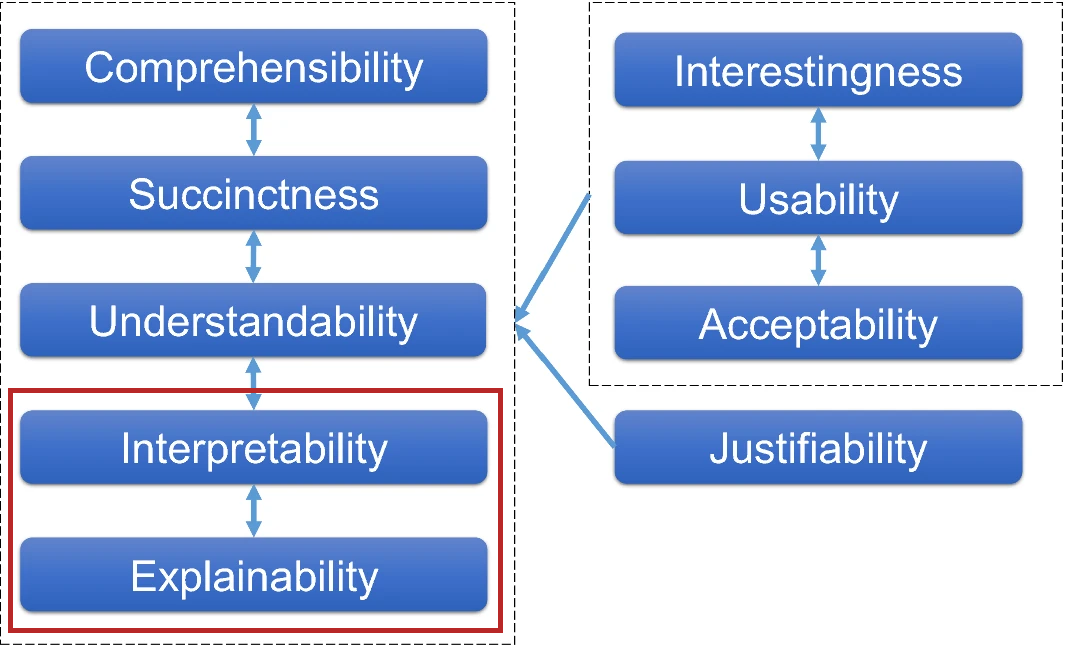
\includegraphics[width=\textwidth]{img/many_words.png}
        \centering
        \caption{Outline of the relationships between the common XAI terminologies}
    \end{figure}    
\end{minipage}
\hfill%
\begin{minipage}[c]{0.65\textwidth}
    In the Explainable AI domains there many terms that seems to be the same meaning.
    Specifically we are interested into two terms: Explainablility and Interpretability.\\
    
    Explainablility provide insights about an AI model while Interpretability tells if the insights make sense to the audience.
\end{minipage}

\subsection{Types of XAI}
\begin{minipage}[c]{0.5\textwidth}
    \begin{figure}[H]
        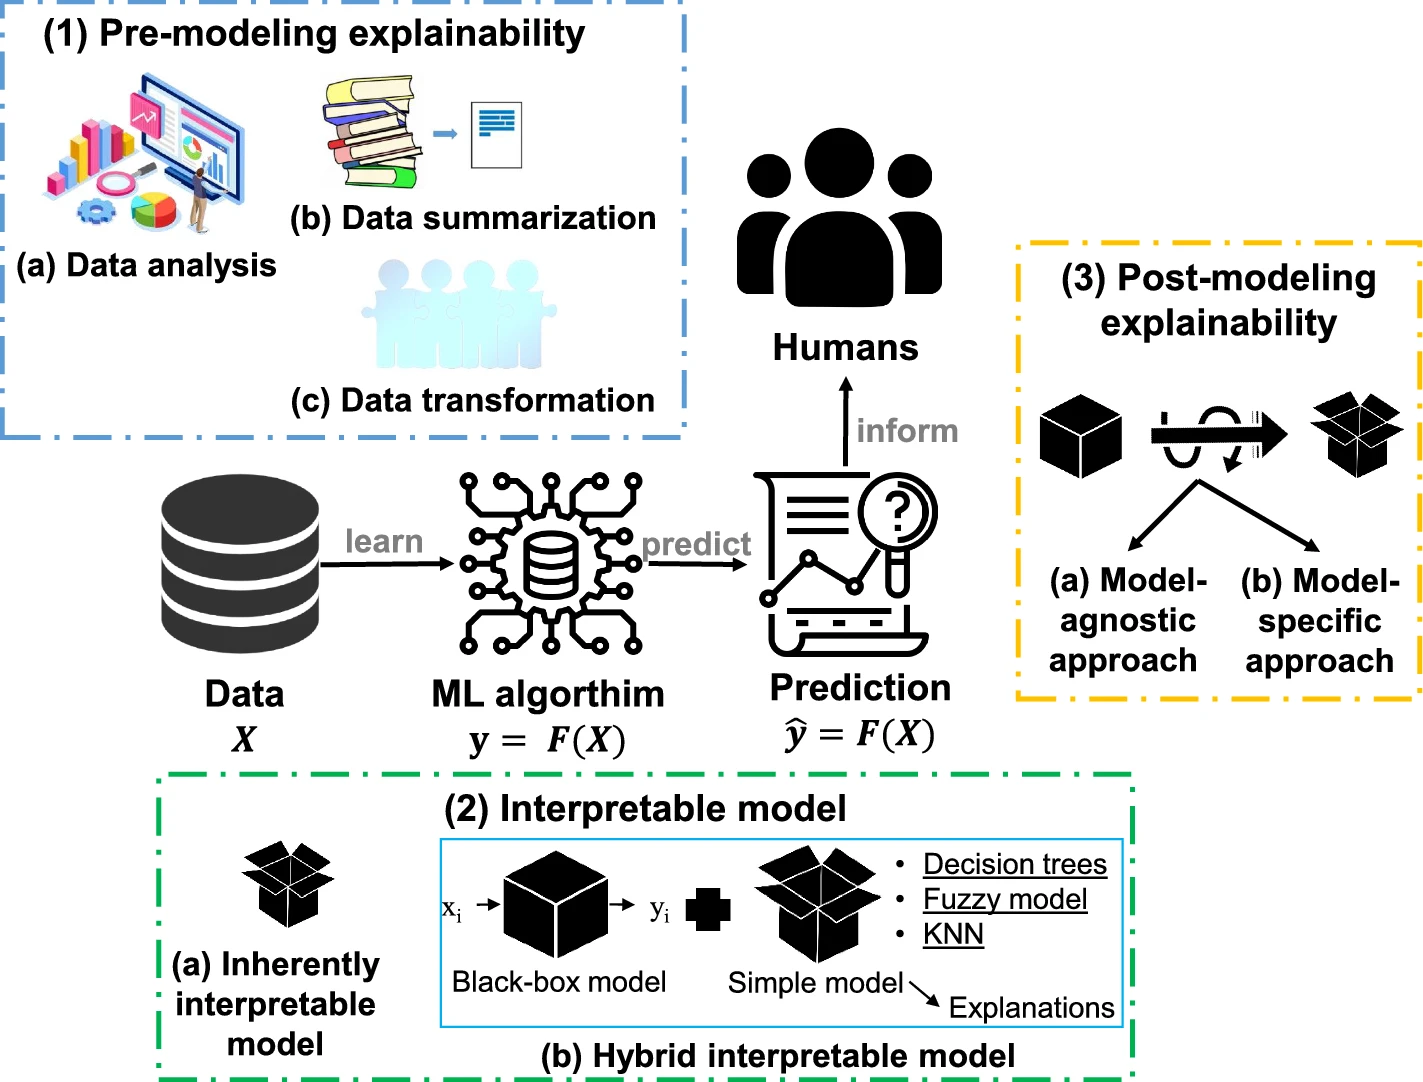
\includegraphics[width=0.8\textwidth]{img/types_XAI.png}
        \centering
        \caption{Outline of the relationships between the common XAI terminologies}
    \end{figure}
\end{minipage}
\begin{minipage}[c]{0.5\textwidth}
    There are three main types of Explainablility:
    \begin{enumerate}
        \item \textbf{Pre-modeling explainability}: summarize input data to identify most relevant features or aspects, based on statistical analysis. Some examples are: K-Means and PCA
        \item \textbf{Post-modeling explainability}: explain the results of a black-box model. Some tecniques include: 
        \begin{itemize}
            \item \emph{Feature relevance}: which input data mostly influences the output?
            \item \emph{Simplification}: aims to make a simplified version of the original model that has an
            optimized function, significantly reduces the complexity, has a simpler implementation
            process, and performance is comparable to the original version.
            \item \emph{Visualization}: interprets a models behavior by visual representations. Visualiza-
            tion techniques are considered the best way to explain the complicated inner interac-
            tions of the variables of the model, and they can be combined with other methods in
            order to increase their interpretability ability.
            \item \emph{Textual justifications}: explains a model by generating explanations in the form of
            text
            \item \emph{Contrastive explanations}: clarifies why an event occurred in contrast to another
        \end{itemize}
        \item \textbf{Interpretable models}: the model is not black-box on its own. some examples include: Linear or logistic regression and Decision trees
    \end{enumerate}
\end{minipage}\\

There are three main properties for interpretability:
\begin{itemize}
    \item Algorithmic transparency: The model can be expressed as a set of known mathematical or logical relations
    \item Decomposability: The model can be decomposed in submodules, with clear indication of connections between them
    \item Simulatability: The model can be easily simulated by a human, given only any input
\end{itemize}